\section{Evaluation}
\label{sec:evaluation}

\begin{table}[t]
\centering
\begin{tabular}{p{0.15\columnwidth} p{0.75\columnwidth}}
\toprule
\textbf{CPU} & 2$\times$Xeon E5-2640v4~2.40~GHz\\
  & 10 cores (20 hardware threads) per socket
\\
\midrule
\textbf{RAM} & 1~TB 2400~MHz DDR4
\\
\midrule
\textbf{NIC} & Mellanox CX5, 40~Gbps Ethernet
\\
\midrule
\textbf{OS} & Ubuntu 16.04, Linux 4.4.0-116,\\
        & DPDK~17.08, 16$\times$1~GB~Hugepages,\\
        & Rust 1.28.0-nightly
\\
\bottomrule
\end{tabular}
\caption{Experimental configuration. Evaluation used
one machine as server and one as client.
Only the NIC-local CPU socket was used on the server.}
\label{table:setup}
\end{table}

We evaluated Splinter on five key questions:

%\begin{description}[leftmargin=0.5em]
%\item[What is Splinter's isolation overhead?]
%\item[Does Splinter support large tenant densities?]
%\item[How does Splinter perform under heterogeneity?]
%\item[How well does a representative extension perform?]
%\end{description}

\begin{enumerate}
\item What is Splinter's isolation overhead?
\item Does Splinter support high tenant densities?
\item How does Splinter perform under operations with heterogeneous runtimes?
\item Do representative extensions see latency and throughput benefits?
\item When does performing operations client-side outperform extension-based operations?
\end{enumerate}

\subsection{Experimental Setup}
All evaluation was done on two machines consisting of one client
and one storage server on the CloudLab
testbed~\cite{cloudlab} (Table~\ref{table:setup}). Both used
DPDK~\cite{dpdk} over Ethernet using Mellanox NICs for kernel-bypass
support. The server was configured to use only one processor socket; out
of the ten hardware cores, eight were used for request processing, one
was used for management and to detect misbehaving extensions, and the
last one was used to hold all misbehaving extensions once detected.

To evaluate Splinter and its isolation costs under high load and density, the
  client ran a YCSB-B workload~\cite{ycsb} (95\% gets, 5\% puts;
  keys were chosen from a Zipfian distribution with $\theta=0.99$) that
  accessed tenant data on the storage server.
Unless stated otherwise, the client simulates 1,024~total tenants.
Tenant ids for each request were chosen from a Zipfian distribution
  with $\theta=0.1$ (unless stated otherwise) to simulate some tenant skew.
Each simulated tenant owns one data table consisting of 1~million 100~B record
  payloads with 30~B primary keys (totaling about 120~GB of stored data).
The client always offered an open-loop load to the server.

\subsection{Isolation Overhead}
\label{sec:isolation-overhead}

%\begin{table}
%  \centering
%  \begin{tabular}{ll}
%    \toprule \textbf{Operation} & \textbf{Latency (ns)} \\
%    \midrule
%    Construct generator & 360 \\
%    Enter/exit extension & 100 \\
%    Database call & 18 \\
%    \bottomrule
%  \end{tabular}
%  \caption{Latency of Splinter's interface.}
%  \label{table:key-ops}
%\end{table}

\begin{figure}[t]
\centering
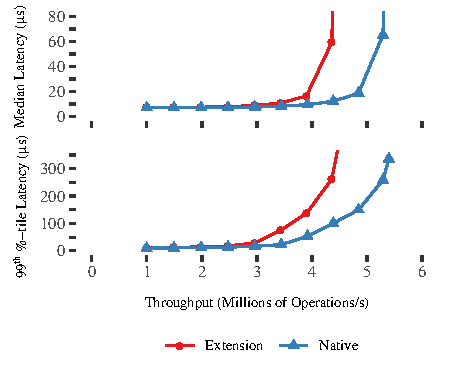
\includegraphics[width=1.0\columnwidth]{graphs/ycsb-open.pdf}
\caption{Comparison of YCSB-B performance using native and extension-based
	\texttt{get()} and \texttt{put()} operations at a tenant density
	of 1,024. When using extensions, the server saturates at
	4.3~million operations per second. In comparison, native
	operations are about 23\% more efficient, saturating at 5.3~million operations
	per second.}
\label{fig:open-load}
\end{figure}


Figure~\ref{fig:open-load} compares the performance of YCSB-B under two
different cases.
In one case (``Native''), the Splinter store executes get and put operations like
  any other key-value store would; none of Splinter's extension functionality
  is used.
This case sets an upper-bound for Splinter's performance.
In the other case (``Extension''), that same get or put is executed as part of a
  tenant-provided and untrusted Splinter extension.
This teases apart the isolation and dispatch costs for Splinter to run
  arbitrary tenant-provided logic.
For offered loads of less than 3.5~million operations per second (Mops/s), median
  latency with and without isolation are nearly identical (about 9~\us).

Splinter extensions have some overhead, so the store saturates
  earlier when gets/puts are executed through extensions.
With isolation, the median latency spikes above 4~Mops/s, reaching 59~\us at
  4.3~Mops/s.
Without isolation, this spike comes at 5.3~Mops/s.
Tail latency (99\textsuperscript{th}-percentile) begins to show a difference at
  3~Mops/s.
On the whole, in this pessimal workload with extremely fine-grained operations
  all invoked as extensions, Splinter's isolation costs still only impact
  throughput of the store by about 19\%.
Compared to the 1.8$\times$ (simulated) penalty for hardware-based
  isolation in Figure~\ref{fig:simulator}, this is a significant
  improvement (a 1.2$\times$ penalty over native get/put).

\begin{figure}[t]
\centering
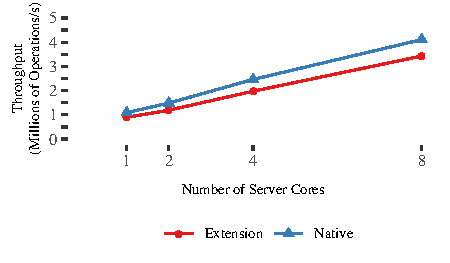
\includegraphics[width=1.0\columnwidth]{graphs/server-scalability.pdf}
\caption{Storage server scalability at a tenant density of 1,024. Points
	represent throughput when YCSB-B latency crosses 10~\us.
	Isolation overhead is consistently lower than 20\%.}
\label{fig:server-scalability}
\end{figure}


Figure~\ref{fig:server-scalability} compares YCSB-B scalability when the server
  is approaching saturation (median latency $>$~10~\us) under the native and
  extension-based cases.
Invoking get and put operations from extensions instead of directly has no
  impact on scalability; scalability is near linear in both scenarios.
However, as pointed out above, it does affect throughput.
At one core, throughput is reduced by 200~Kops/s (18\%), while at eight cores,
  the reduction is 700~Kops/s (17\%).
This shows that, though extensions do increase the number of cycles each core
  spends processing requests, it doesn't come at the cost of significant
  increased coordination between the cores.

\subsection{Tenant Density}

\begin{figure}[t]
\centering
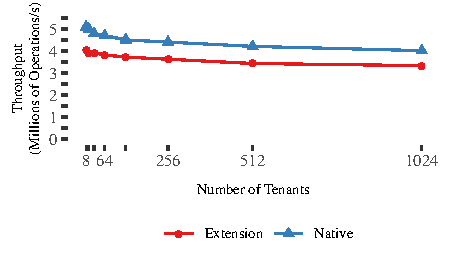
\includegraphics[width=1.0\columnwidth]{graphs/tenant-scalability.pdf}
\caption{Scaling tenants. Points represent server
	throughput when YCSB-B latency crosses 10~\us.
	With isolation, increasing the number of
	tenants only impacts performance modestly; moving from 8 to 1,024 tenants
	reduces throughput by 700~Kops/s.}
\label{fig:tenant-scalability}
\end{figure}


Figure~\ref{fig:tenant-scalability} shows how varying the number of tenants
  sharing the store impacts its throughput.
As in the prior experiments, tenants run YCSB-B under two cases:
without isolation (``Native'') and with isolation (``Extension''), so the
experiment captures extension isolation
  overheads.
The results show that Splinter can efficiently support high tenant densities
  with minimal overhead.
With isolation, the throughput at 1,024 tenants is 3.3~Mops/s, only
700~Kops/s less than the throughput at 8 tenants. Additionally,
the throughput with isolation is consistently within 22\% of the throughput
without isolation.

%Splinter's tenant scalability
%when the storage server is close to saturation under YCSB.
\begin{figure}[t]
\centering
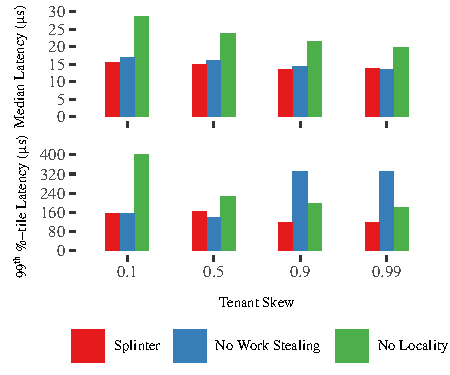
\includegraphics[width=1.0\columnwidth]{graphs/tenant-skew.pdf}
\caption{Latency with tenant skew. The server runs
	near saturation at 4~Mops/s in each case. Without work
	stealing, tail latency under high skew increases from 138~\us to
	330~\us. Without tenant locality, median and tail latencies
	are affected.}
\label{fig:tenant-skew}
\end{figure}


In practice, offered tenant load will be skewed, since some tenants are likely
  to have heavier workloads than others.
This results in a few heavy workloads that must share the store with a long
  tail of many more passive ones.
We ran an experiment to show that Splinter can handle this imbalance and
  that its work stealing and tenant locality help maintain Splinter's
  response times under high load.

Recall that Splinter routes requests for a tenant to a specific
  core, but cores steal work from each other to combat imbalance.
To gauge the benefits of this approach, we compare it against a tenant-partitioned
  approach with no work stealing and an unpartitioned approach that sprays
  requests over all cores in a tenant-oblivious fashion.
We vary tenant skew, which affects all three approaches.

Figure~\ref{fig:tenant-skew} shows the results.
These measurements are with an offered load of 4~Mops/s, keeping the
  store close to saturation.
In each case, the store meets the offered load by running at
  4~Mop/s.
Without work stealing, Splinter's tail latency suffers by a factor of 2 under
  high tenant skew (0.9 and 0.99).
In this case, partitioning helps throughput due to locality and reduced
  contention (as evidenced by its relatively consistent median response time),
  but queues become imbalanced hurting tail latency.
The unpartitioned approach doesn't respond as significantly to tenant skew
  though it is slower overall, as expected.
Unpartitioned execution results in
  42\% to 86\% worse median latency with 38\% to 155\% worse tail latency.
%In this case, work is more homogeneous across the cores, which avoids idling and
%  is more resilient to skew, but increased coordination costs slow the store.

\subsection{Request Heterogeneity}

\begin{figure}[t]
\centering
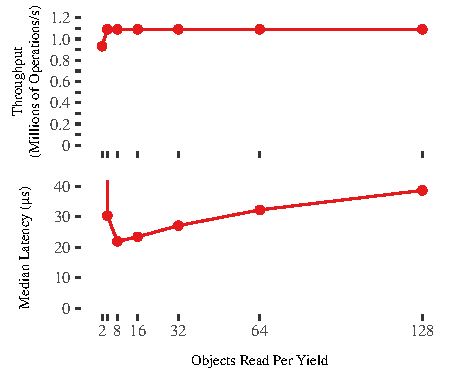
\includegraphics[width=1.0\columnwidth]{graphs/long-cooperative.pdf}
	\caption{Performance with a small fraction (15\%) of cooperative long
	running procedures that perform 128 \texttt{get}s. Yielding
	frequently can help improve median latency from 38~\us to
	22~\us. However, yielding
	too frequently hurts median latency. The storage server was
	offered a constant load of 1.1~Mops/s.}
\label{fig:long-cooperative}
\end{figure}


Figure~\ref{fig:long-cooperative} investigates the impact of mixing short operations
with cooperative longer-running operations.
We configured our client so that
15\% of extension operations performed
128 \texttt{get}s on the storage server. The rest of the
requests invoked an extension that performed one \texttt{get}.
We varied the number of \texttt{get}s made by the longer
extension per yield (frequency).
These measurements were made at an offered load of 1.1~Mops/s.
Increasing the frequency of yields improves median
latency of the smaller operations by 42\% until a frequency of 8 \texttt{get}s per
yield.
Yields add some overhead, and yielding more frequently pushes the store to
  saturation in this case.
As a result, all requests see increased response times.
Extensions should yield frequently, but
yielding too often is wasteful.
Splinter may be able to help with this in the future; Splinter could provide
  extensions with a yield that is ignored if called too quickly in succession,
  avoiding the full yield cost.

\begin{figure}[t]
\centering
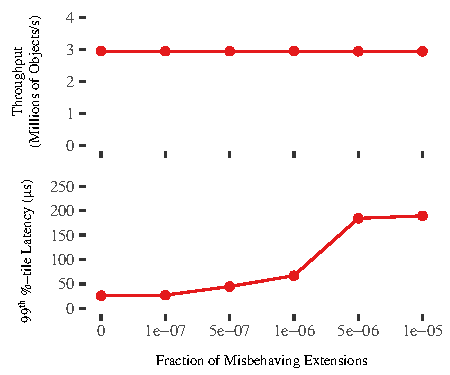
\includegraphics[width=1.0\columnwidth]{graphs/uncooperative.pdf}
\caption{Impact of uncooperative requests on performance. System
	throughput stays constant at 3~Mops/s throughout. For fractions
	of uncooperative requests greater than 1 every million, tail
	latency is significantly affected (> 100~\us).}
\label{fig:uncooperative}
\end{figure}


Figure~\ref{fig:uncooperative} shows how uncooperative
  extensions impact system performance. Here, the client invoked a
  small fraction of extension operations that executed an infinite
  loop.
The remaining fraction of requests invoked a small extension that performed a
  single \texttt{get}.
Splinter performs well in the presence of misbehaving extensions.
Throughput is steady at 3~Mops/s
  irrespective of the fraction of misbehaving requests.
Median latency isn't shown, but it is steady as well.
Tail latency suffers as more requests misbehave, though it is within
  100~\us for fractions as high as one in a million requests.

Note that one in a million requests (1e-6) is harsh.
The store can execute more than 4 Mop/s, so this represents a misbehaving
  invocation starting every quarter second; at 1e-5 misbehavior starts about once
  every 25~ms.

\subsection{Aggregation Extension}
\label{sec:eval-agg}

\begin{figure}[t]
\centering
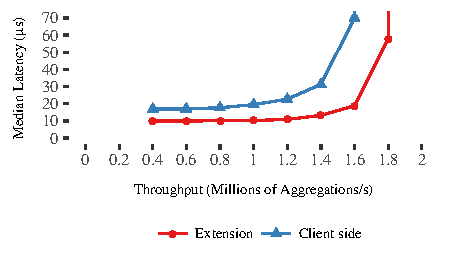
\includegraphics[width=1.0\columnwidth]{graphs/aggregate.pdf}
  \caption{Aggregation throughput versus latency. Aggregations
    combine four records. Under low
    load, the median latency of a client-side implementation is 1.6$\times$
    that of an extension-based implementation. Using an
    extension also improves saturating throughput from 1.2~M to 1.6~M
    aggregations per second.}
\label{fig:aggregate-bench}
\end{figure}


Online data aggregation is a common task for applications.
For example, a user might send a query
  demanding a movie studio's total earnings in the year 2017.
With a key-value data model, this would require two
  round-trips to storage:
one to fetch the list of movies made
  by the studio and one to fetch the box-office earnings of each
  of the movies.
Splinter improves the user-facing and server-side performance of these types of
  queries by allowing applications to inexpensively embed their data model
  (studios and movies) and operations (total earnings aggregation) within
  storage.

Figure~\ref{fig:aggregate-bench} compares a completely client-based and a
  Splinter extension-based implementation of such an aggregation over 4
  records.
Each of the store's 1,024 tenants owned a table with 300~K
  indirection lists pointing to 1.2~million records, totalling about 100~GB of
  stored data.
The client-based implementation first performed a \texttt{get()} to
  retrieve an indirection list followed by a \texttt{multiget()} (a single RPC
  requesting values for multiple keys) to fetch all of the records indicated in
  the indirection list.
The first field from each of the returned objects is summed up into a single
  64-bit result.
The extension-based implementation invoked a Splinter extension called
  \texttt{aggregate()} with the same functionality as the client-based approach.

Pushing the aggregation from the client to the server has two key benefits.
First, it improves performance from the client's perspective: the
  extension-based implementation reduces median latency by 38\% (from
  16~\us to 10~\us) under low load with larger gains under higher loads.
This improvement is mainly due to a reduction in the number of round-trips;
unlike the client-based extension, the \texttt{aggregate()} extension doesn't
  need to wait for the store to return an indirection list before it can start
  aggregation.
Second, it improves performance from the server's perspective as well.
Splinter's extension invocations are more expensive than plain \texttt{get()}
  operations (\S\ref{sec:isolation-overhead}), but they eliminate
  some of the costly network and RPC processing.
Hence, saturating throughput improves from 1.2~M to 1.6~M aggregations
  per second.

Note, this improvement comes in a challenging case for Splinter; at 40~Gbps,
  Splinter is never network limited.
These results show that even if a store is CPU-limited, pushing compute to the
  store can still provide a throughput benefit, since it can mitigate
  request processing overheads.
On slower networks, Splinter would provide more of a benefit since extensions
  can reduce network load.

\begin{figure}[t]
\centering
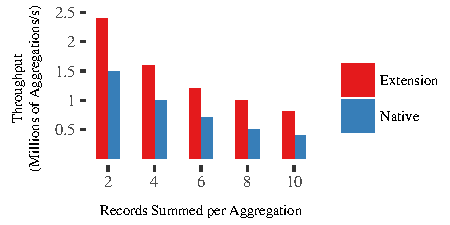
\includegraphics[width=1.0\columnwidth]{graphs/aggregate-sum-throughput.pdf}
  \caption{Saturating throughput of aggregation versus the
    number of aggregated records. The extension-based implementation
    outperforms the client-side implementation irrespective of the
    number of records aggregated. The gains are highest when
    aggregations are over two records (2.4~M versus 1.5~M aggregations per second).}
\label{fig:aggregate-sum-sizes}
\end{figure}


\begin{figure}[t]
\centering
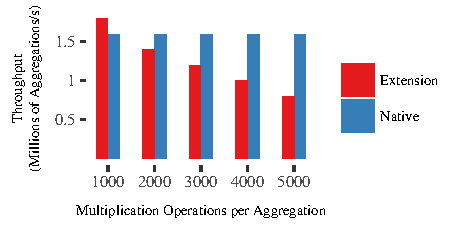
\includegraphics[width=1.0\columnwidth]{graphs/aggregate-mul-throughput.pdf}
  \caption{Saturating throughput of the aggregation extension versus the
    amount of compute per aggregation. After aggregating 2 records, each
    operation raised the result to the power \texttt{n}, implemented as
    \texttt{n} 64-bit multiplications (hence the x-axis). Increasing the
    order (\texttt{n}) increases server-side compute in the
    extension-based implementation, hurting throughput. At an order of
    5000, the client-side approach is 2$\times$ faster.}
\label{fig:aggregate-mul-sizes}
\end{figure}


Figure~\ref{fig:aggregate-sum-sizes} shows the impact of the number of
  records aggregated on the saturating throughput of the extension-based
  and client-based implementation.
In both approaches, increasing the number of records aggregated
  increases the work the store has to do per request
  (\texttt{aggregate()/multiget()}), and, hence, decreases the overall
  throughput of the system. 
However, if that work is simple (like summation) it is always better to
  aggregate at the store.
%However, the extension-based approach continues to receive a performance boost
%  from the reduced round-trips unlike it's client-based counterpart.
The gain in saturating throughput of the extension-based aggregation is
  always more than 50\%.

For compute-intensive operations, the extra CPU cost of
running extensions at the store can outweigh the gains of fewer RPCs.
Figure~\ref{fig:aggregate-mul-sizes} explores this effect.
After adding the first field of two records, each operation raises the
  result to the power \texttt{n} (with \texttt{n} 64-bit
  multiplications).
Using an extension, increasing \texttt{n} above 2,000
  slows the store and decreases
  saturating throughput from 1.8~M to 800~K aggregations per second.
The client-side approach can hold throughput constant
  at 1.6~M aggregations per second;
the client has enough idle CPU capacity to compute the result.
This shows that extensions are ideal for operations with
  modest amounts of compute.
For compute-intensive operations over data stored on high-load servers,
  clients should fetch data and perform operations locally.

\subsection{TAO Extension}

\begin{figure}[t]
\centering
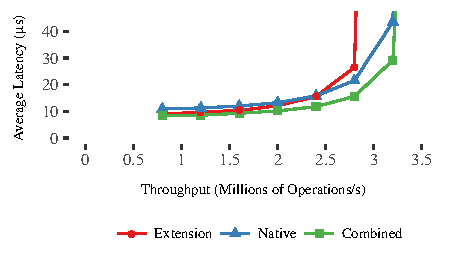
\includegraphics[width=1.0\columnwidth]{graphs/tao.pdf}
  \caption{TAO extension throughput versus latency. With 60\%
    \texttt{object\_get} and 40\% \texttt{assoc\_range} operations,
    the TAO extension can reach 2.8~Mop/s
    before saturating with an average latency of 30~\us. By using
    native \texttt{get()} operations for \texttt{object\_get}, the
    extension-based approach can outperform a purely client-side
    implementation by 400~Kop/s.}
\label{fig:tao-bench}
\end{figure}


TAO~\cite{tao-2013} is a graph-oriented in-memory cache used at Facebook to hold
  objects from the social graph and associations between those objects.
TAO is well-suited to Splinter.
It is designed for interactive data, but it embeds knowledge
  about Facebook's workload to decrease round-trips to the store, which
  eliminates client-side stalls and improves server-side efficiency.
We have implemented its simple operations as an 800-line Splinter extension.

Full details of TAO are beyond the scope of this paper, but the basics are
  simple. Aside from object put/get, TAO's \textsl{association lists} (e.g.\
  \texttt{user1}'s ``likes'') allow one object to be
  associated to another via a typed, directed edges.
For example, \texttt{user1}'s ``likes'' may be represented as an association list
  \texttt{(user1, likes)} $\rightarrow$ [\texttt{post1}, \texttt{post32}].
Association lists provide simple operations for adding, removing, and counting
  associations. Entries in association lists are timestamped, and range operations
  over association lists to fetch subsets of them are common (``get the first 10 entries in
  the \texttt{(user1, likes)} association list'').

Figure~\ref{fig:tao-bench} shows Splinter's performance under three
different configurations: an extension-based approach (Extension), a
client-based approach (Native), and a combined approach (Combined) that implemented
\texttt{object\_get} using native \texttt{get()} operations, and
\texttt{assoc\_range} using an extension.
The workload was configured to
issue a mix of 60\%
  \texttt{object\_get} and 40\% \texttt{assoc\_range} operations.
We picked this ratio based on Facebook's reported TAO workload~\cite{tao-2013},
  which is dominated by reads (99.8\%) mostly from these two operations.
Each of the 1,024 tenants on the storage node owned a graph with half a million
  objects and two million edges (associations), totalling about 100~GB of
  stored data.

Since a significant fraction of requests are single round-trip
\texttt{object\_get}s, the client-based approach has a better
saturating throughput than the extension-based approach. However,
combining the two improves
saturating throughput from 2.8~Mop/s to 3.2~Mop/s at a latency of
31~\us;
the native \texttt{get()} helps eliminate the isolation
overhead while executing an \texttt{object\_get}, and the extension helps
reduce the number of round-trips required by an \texttt{assoc\_range}.

This makes Splinter competitive with FaRM's TAO implementation which is the
  fastest known implementation.
Interestingly FaRM, takes the opposite approach of Splinter.
On FaRM, TAO operations use multiple RDMA reads and careful
  object layout.
FaRM reported 6.3 Mops/s (about 200 Kop/s/core) with a 41~\us average latency;
  Splinter performs about 400 Kops/s/core with lower latency.
Differences in hardware and experimental setup likely account for some
  of the differences, but it shows Splinter's CPU-active server approach
  is competitive against FaRM's CPU-passive server approach.
Furthermore, Splinter maintains a simple, remote procedure call interface, and
the TAO extension enforces strong abstract data types.
Splinter TAO clients have no knowledge of the internal layout of the stored
  data objects.
